\documentclass[12pt]{article}
\usepackage{amsmath}
\usepackage[margin=1 in]{geometry}
\usepackage{graphicx}
\usepackage{booktabs}
\usepackage{natbib}
\usepackage{lipsum}
\usepackage[colorlinks=true, citecolor=blue]{hyperref}

\title{STAT3494}
\author{Julia Andronowitz\\
University of Connecticut}
\date{September 26, 2022}

\begin{document}
\maketitle

\begin{abstract}

This will contain the abstract for my paper.
\lipsum[2]

\end{abstract}

\section{Introduction}

What is the topic and why is it worth studying? - the first major section of text in the paper, the Introduction commonly describes the topic under investigation, summarizes or discusses relevant prior research (for related details, please see the Writing Literature Reviews section of this website), identifies unresolved issues that the current research will address, and provides an overview of the research that is to be described in greater detail in the sections to follow.

\lipsum[1]

To cite a reference, here are examples.
\citet{xie2015dynamic} did something ... \lipsum[4]

A lot of work has been done \citep[e.g.,][]{xie2015dynamic}.

\lipsum[2]

\section{Data}

\begin{equation}
  \label{eq:mc2}
  E= m c^2
\end{equation}

\lipsum[3]


\section{Methods}

What did you do? - a section which details how the research was performed.  It typically features a description of the participants/subjects that were involved, the study design, the materials that were used, and the study procedure.  If there were multiple experiments, then each experiment may require a separate Methods section.  A rule of thumb is that the Methods section should be sufficiently detailed for another researcher to duplicate your research.

\begin{equation}
	\label{eq:area}
	\pi r^2
\end{equation}

Equation~\eqref{eq:area} is the area of a circle. Below is an unnumbered equation.

\[
f(x)=\frac{1}{\sqrt{3\pi}}\exp
\]

\section{Results}

What did you find? - a section which describes the data that was collected and the results of any statistical tests that were performed.  It may also be prefaced by a description of the analysis procedure that was used. If there were multiple experiments, then each experiment may require a separate Results section.

Table~\ref{tab:rv} summarizes some example draws from some distributions.

\lipsum[1-4]

\begin{table}[ht]
  \caption{This is a table of some distributions.}
  \label{tab:rv}
\centering
\begin{tabular}{rrr}
  \toprule
normal & poisson & gamma \\ 
  \midrule
-0.110 & 4 & 2.401 \\ 
  0.116 & 4 & 3.529 \\ 
  -0.828 & 9 & 2.112 \\ 
  -0.066 & 6 & 11.104 \\ 
  0.219 & 3 & 4.815 \\ 
  0.303 & 5 & 2.188 \\ 
  0.544 & 0 & 8.050 \\ 
  -2.617 & 8 & 3.646 \\ 
  0.747 & 1 & 5.178 \\ 
  -1.103 & 4 & 3.043 \\ 
   \bottomrule
\end{tabular}
\end{table}

Figure~\ref{fig:cars} shows the distance against the speed from this dataset.

\begin{figure}
  \centering
  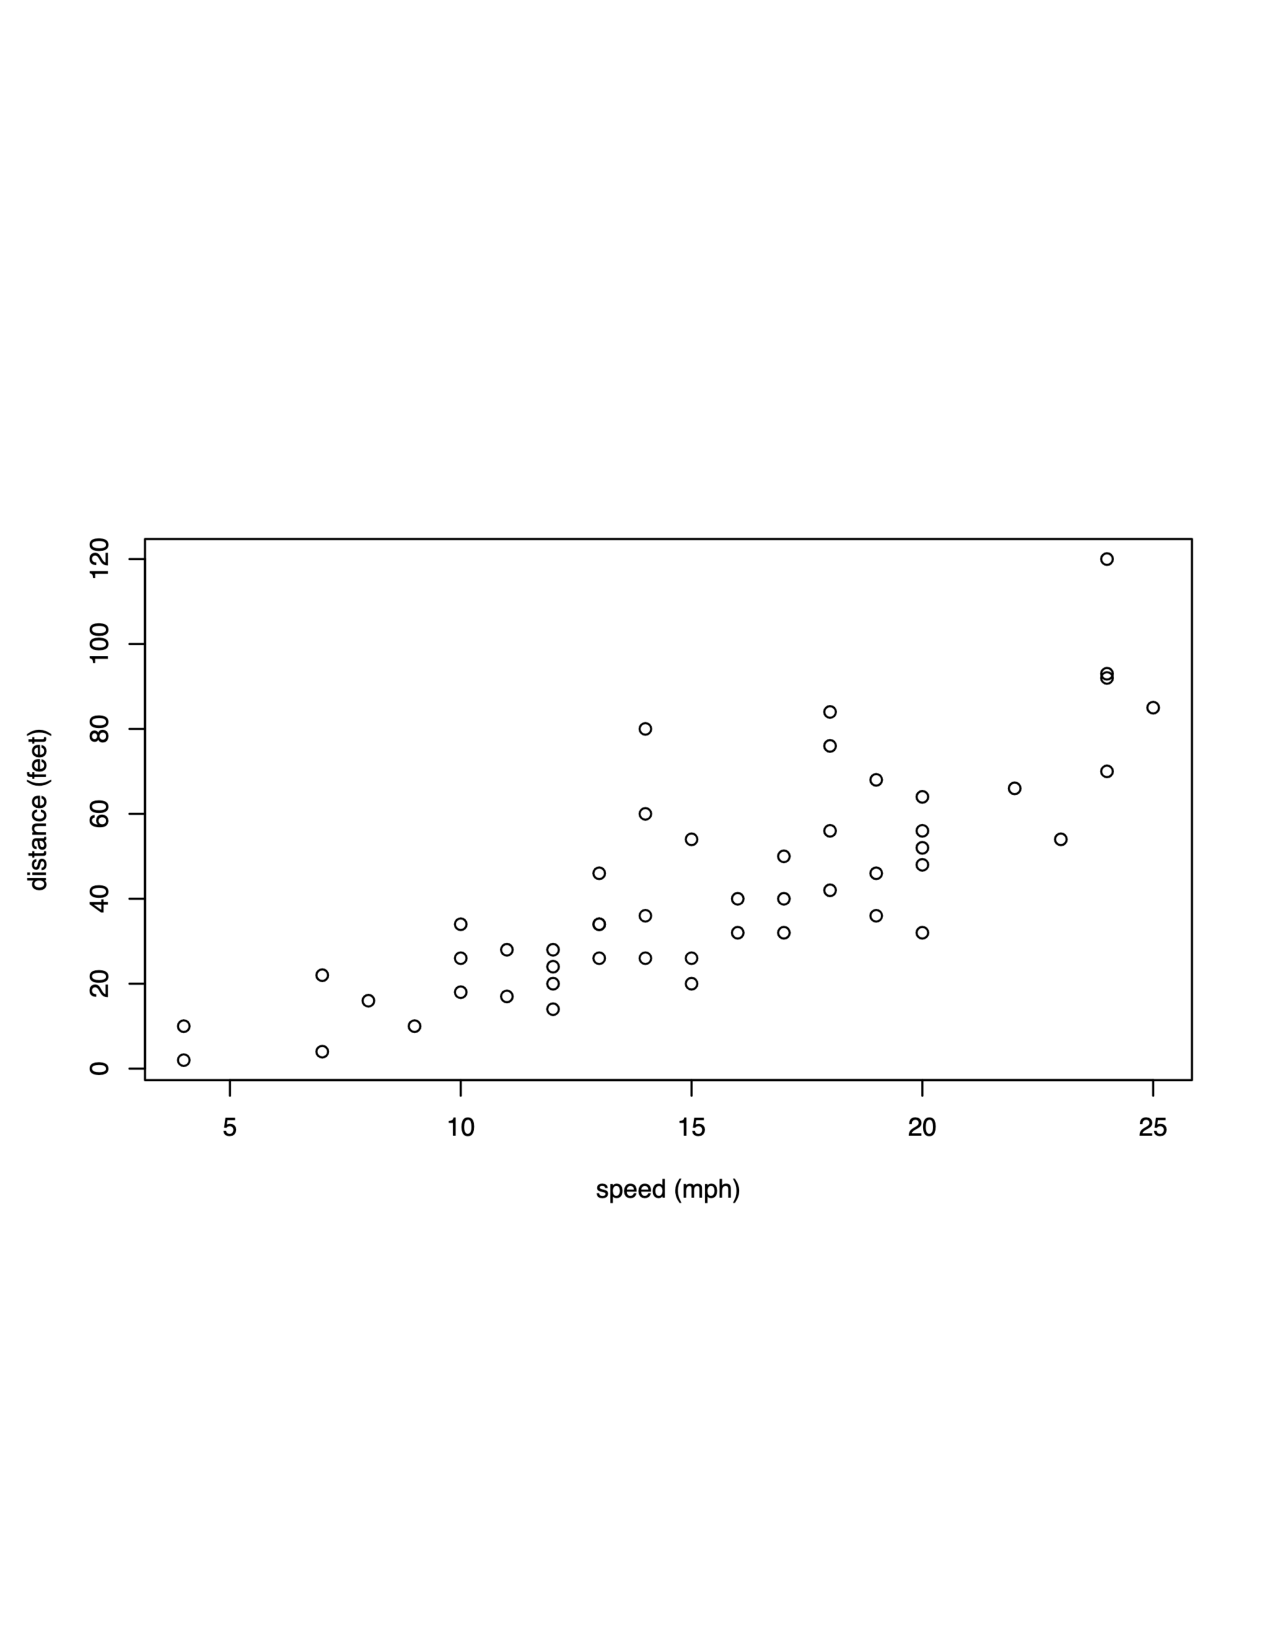
\includegraphics[width=\textwidth]{cars.pdf}
  \caption{This is a figure of the cars.pdf}
  \label{fig:cars}
\end{figure}

\section{Discussion}
What is the significance of your results? - the final major section of text in the paper.  The Discussion commonly features a summary of the results that were obtained in the study, describes how those results address the topic under investigation and/or the issues that the research was designed to address, and may expand upon the implications of those findings.  Limitations and directions for future research are also commonly addressed.

Another citation \citep{srinath2017python}.

\bibliography{references}
\bibliographystyle{chicago}

\end{document}
